\documentclass[tikz, border=6pt]{standalone}
\usepackage{tikz}
\usetikzlibrary{shapes.geometric, arrows.meta, positioning}

\tikzset{
  io/.style={
    trapezium, trapezium left angle=75, trapezium right angle=105,
    draw, thick, fill=black!10,
    text centered, minimum width=2.2cm, minimum height=0.45cm,
    font=\scriptsize
  },
  process/.style={
    rectangle, draw, thick, fill=white,
    text centered, minimum width=2.2cm, minimum height=0.45cm,
    font=\scriptsize
  },
  model/.style={
    rectangle, draw, very thick, fill=black!20,
    text centered, minimum width=2.2cm, minimum height=0.5cm,
    font=\scriptsize\bfseries
  },
  decision/.style={
    diamond, draw, thick, fill=black!5,
    text centered, minimum width=1.5cm, minimum height=0.45cm,
    inner sep=0pt, font=\tiny
  },
  mapping/.style={
    rectangle, draw, thick, fill=black!8,
    text centered, minimum width=2.2cm, minimum height=1.0cm,
    font=\tiny
  },
  discard/.style={
    rectangle, draw, thick, dashed, fill=black!5,
    text centered, minimum width=1.4cm, minimum height=0.38cm,
    font=\tiny
  },
  output/.style={
    rectangle, draw, very thick, fill=black!30, text=white,
    text centered, minimum width=2.2cm, minimum height=0.5cm,
    font=\scriptsize\bfseries
  },
  arr/.style={-{Stealth[length=4pt]}, thick},
  darr/.style={-{Stealth[length=3.5pt]}, thick, dashed},
}

\begin{document}
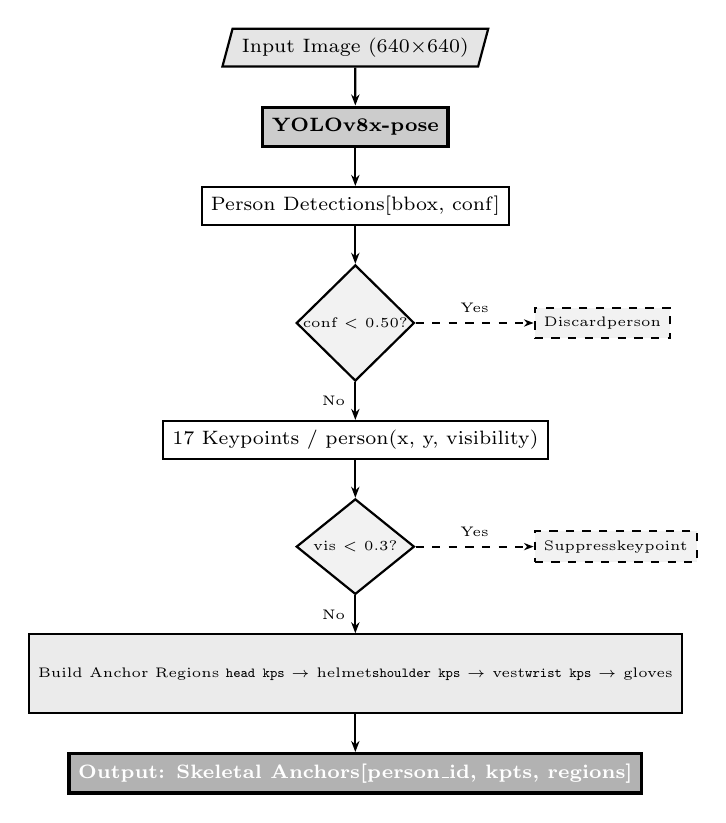
\begin{tikzpicture}[node distance=0.48cm and 1.5cm]

  \node[io]       (input)   {Input Image (640$\times$640)};
  \node[model,    below=of input]   (pose)    {YOLOv8x-pose};
  \node[process,  below=of pose]    (persons) {Person Detections\\{[bbox, conf]}};
  \node[decision, below=of persons] (dconf)   {conf $<$ 0.50?};
  \node[process,  below=of dconf]   (kpts)    {17 Keypoints / person\\(x, y, visibility)};
  \node[decision, below=of kpts]    (dvis)    {vis $<$ 0.3?};
  \node[mapping,  below=of dvis]    (anchor)  {%
    Build Anchor Regions\\[2pt]
    \texttt{head kps} $\rightarrow$ helmet\\
    \texttt{shoulder kps} $\rightarrow$ vest\\
    \texttt{wrist kps} $\rightarrow$ gloves
  };
  \node[output,   below=of anchor]  (out)     {Output: Skeletal Anchors\\{[person\_id, kpts, regions]}};

  \node[discard, right=of dconf]   (disc1)   {Discard\\person};
  \node[discard, right=of dvis]    (disc2)   {Suppress\\keypoint};

  \draw[arr] (input)   -- (pose);
  \draw[arr] (pose)    -- (persons);
  \draw[arr] (persons) -- (dconf);
  \draw[arr] (dconf)   -- node[left, font=\tiny]{No}  (kpts);
  \draw[arr] (kpts)    -- (dvis);
  \draw[arr] (dvis)    -- node[left, font=\tiny]{No}  (anchor);
  \draw[arr] (anchor)  -- (out);
  \draw[darr](dconf)   -- node[above, font=\tiny]{Yes} (disc1);
  \draw[darr](dvis)    -- node[above, font=\tiny]{Yes} (disc2);

\end{tikzpicture}
\end{document}
